\chapter{実験内容}
\section{モデルによる違い}
本研究ではMagentaで用意されている2つの学習モデルを用いた.以下に示すモデルを用いて楽曲制作をそれぞれ行い,比較,検証する.
\subsection{MelodyRNN}
MelodeRNNは楽曲のメロディを制作するモデルである.MelodyRNNである3つのモデルを以下に示す.\\
(1) basic\_rnn\\
 前の状態を保持し,これを記憶または忘却する.時系列を学習することにより,次の音の予測を可能にしている.Lookback\_rnnとAttention\_rnnはこれを基に機能を追加したものである.
\begin{figure}[!ht]
    \begin{screen}
    \begin{center}
        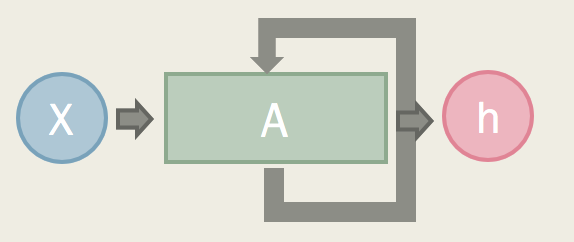
\includegraphics[scale=1.4,clip]{./img/basic3.png}
        \caption{basic\_rnnのモデル(1)}
        \label{fig:basicrnnのモデル(1)}
    \end{center}
    \end{screen}
\end{figure}
\newpage
\begin{figure}[!ht]
    \begin{screen}
    \begin{center}
        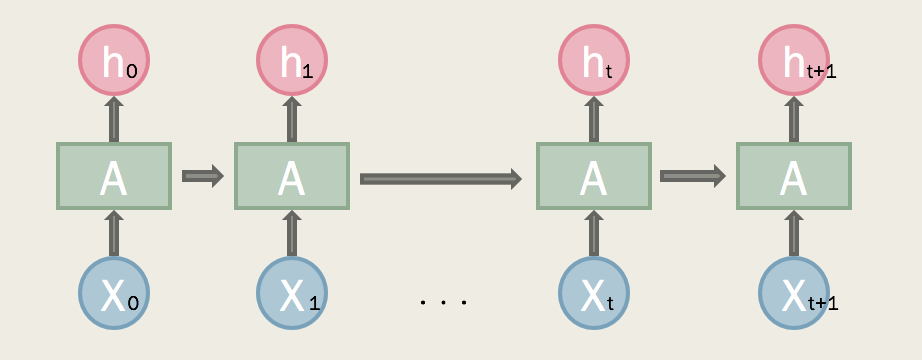
\includegraphics[scale=0.9,clip]{./img/basic4.png}
        \caption{basic\_rnnのモデル(2)}
        \label{fig:basic_rnnのモデル(2)}
    \end{center}
    \end{screen}
\end{figure}
\begin{figure}[!ht]
    \begin{screen}
    \begin{center}
        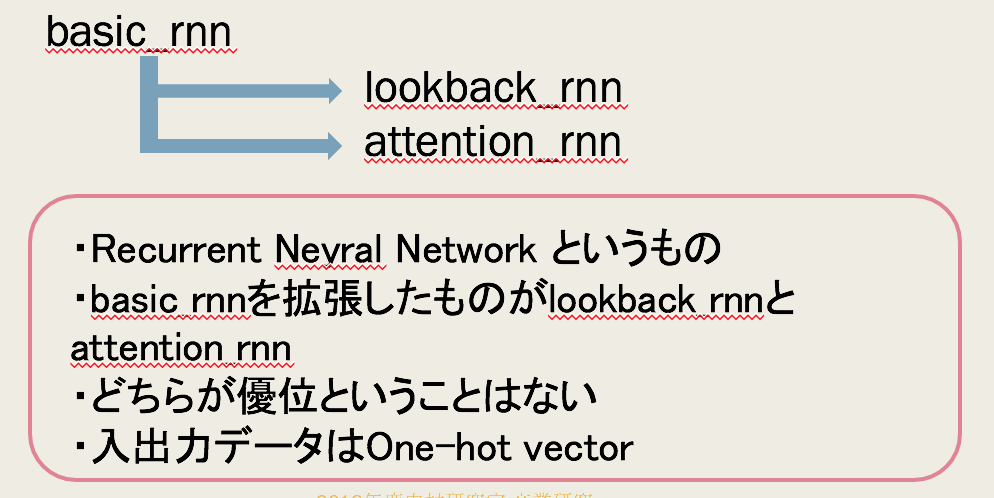
\includegraphics[scale=0.8,clip]{./img/basic1.png}
        \caption{三つのモデルについて}
        \label{fig:Melody_RNNについて}
    \end{center}
    \end{screen}
\end{figure}
\newpage
(2) lookback\_rnn\\
 basic\_rnnを基に,1小節前と2小節前の音,拍数,前の小節の繰り返しかどうかの情報を与え,音楽の流れを掴もうとするものである.これは音楽は繰り返しが多いという特性からなるものであり,これを活かして楽曲生成を行うものである.
\begin{figure}[!ht]
    \begin{screen}
    \begin{center}
        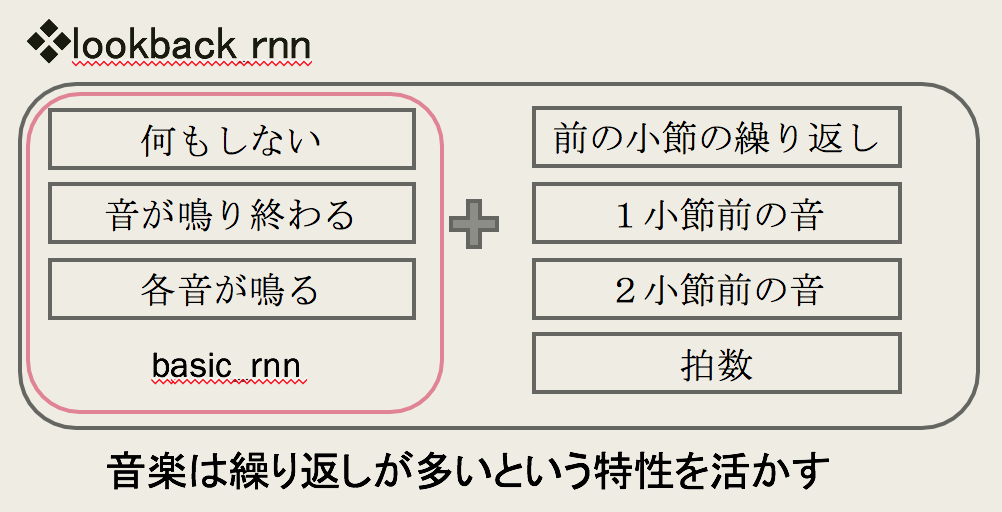
\includegraphics[scale=0.8,clip]{./img/lookback1.png}
        \caption{lookback\_rnnのモデル}
        \label{fig:lookback_rnnのモデル}
    \end{center}
    \end{screen}
\end{figure}
\newpage
(3) attention\_rnn\\
 basic\_rnnを基に,過去の情報を予測結果に加えてこれによる繰り返しを捉えるものである.図\ref{fig:attentio_rnnのモデル}のような流れになっている.
\begin{figure}[!ht]
    \begin{screen}
    \begin{center}
        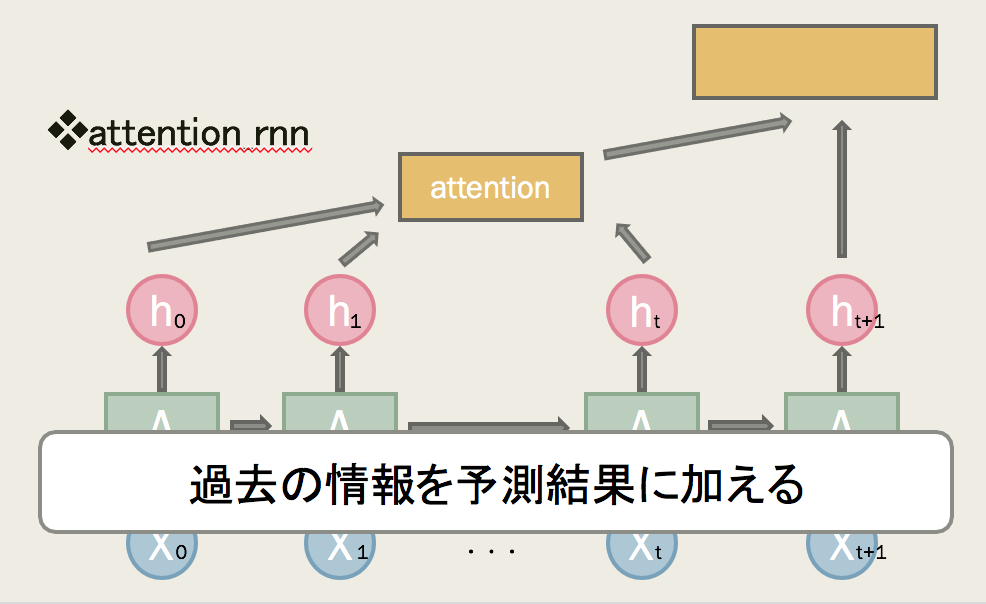
\includegraphics[scale=0.8,clip]{./img/attention1.png}
        \caption{attention\_rnnのモデル}
        \label{fig:attentio_rnnのモデル}
    \end{center}
    \end{screen}
\end{figure}
\subsection{PolyphonyRNN}
 複数の同時音のモデリングが可能になっており,複数音の響きを1つのかたまりとして捉えて学習しているモデルである.このモデルを使用することで,伴奏も含めた楽曲の生成が可能である.\\
 以上のモデルを用いて楽曲制作を行い,それぞれの違いと有用性について検証する.
\newpage
\section{学習回数による違い}
学習回数を変更して楽曲制作を行う.本研究では500回,5000回,20000回でMelodyRNNのbasic\_rnn,lookback\_rnn,attention\_rnnでそれぞれ楽曲を制作した.
これらの結果,生成された楽曲の音程やリズムへの影響やそれぞれの違いを検証し,有用性について検討する.
\section{ノード数による違い}
ノード数を変更して楽曲制作を行う.本研究では32,64,128でbasic\_rnnそれぞれ楽曲を制作した.これらの結果,生成された楽曲の音程やリズムへの影響やそれぞれの違いを検証し,有用性について検討する.